\chapter{Convolutional Neural Network}
Convolutional Neural Networks (CNNs) are similar with the original of Neural Networks. Neural Networks receive an input and pass it through a series of hidden layer. Each hidden layer is made from a set of neurons, where each neuron is full connected with all neurons of previous layer. Actually, the neural networks do not scale well to full images...
\section{Architecture}
A CNN is made from the layers. The common layers in CNN are convolutional, nonlinear, pooling and full connected layers. CNN takes image as an input, pass it through the series of layers and get an ouput. Each layer has a difference function to transform the input to another layer. 
\begin{figure}[h]
	\centering
	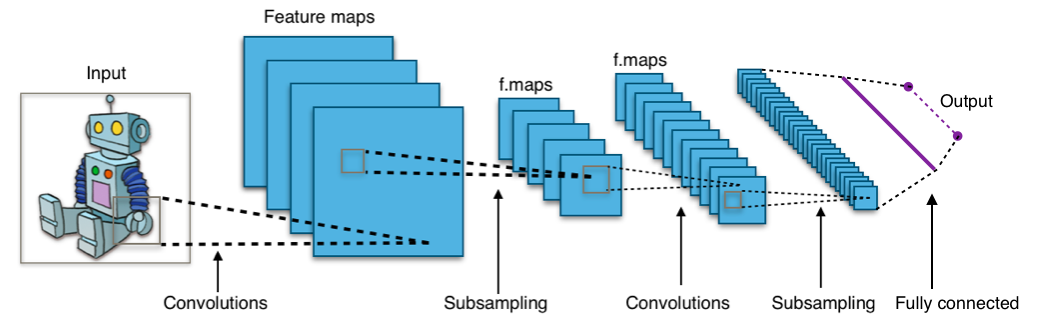
\includegraphics[scale=0.45]{images/cnn_architecture}
	\caption{An architecture of convolutional neural network}
	\label{figlncex}
\end{figure}~\\
\subsection{Convolutional layer}
\subsection{Pooling layer}
\subsection{Full connected layer}
\section{Testing}